\section{Рабочий проект}
\subsection{Классы, используемые при разработке сайта}

\subsubsection{Класс Game}

Класс Game относится к platformer и используется для управления программной системой.

Описание методов класса Game представлено в таблице \ref{table:game_methods}.
\renewcommand{\arraystretch}{0.8} % уменьшение расстояний до сетки таблицы
\begin{xltabular}{\textwidth}{|X|X|}
	\caption{Методы класса Game}\label{table:game_methods} \\
	\hline \centrow
	Название метода & \centrow  Описание метода \\
	\hline \centrow 1 & \centrow 2 \\ \hline
	\endfirsthead
	\continuecaption{Продолжение таблицы \ref{table:game_methods}}\\
	\hline \centrow 1 & \centrow 2 \\ \hline
	\finishhead
	add\_object(self, obj) & Добавляет объект obj в игру,параметр obj: добавляемый объект. \\
	\hline
	remove\_object(self, obj) & Удаляет объект obj из игры, параметр obj: удаляемый объект. \\
	\hline
	clear(self) & Удаляет все игровые объекты. \\
	\hline
	key\_pressed(self, key) & Возвращает True если была нажата клавиша key, иначе False, параметр key: нажимаемая кнопка. \\
	\hline
	new\_state(self, name, first\_func, func) & Создание нового игрового состояния, параметр name: имя состояния, параметр first\_func:функция, которая запускается при переключении в это игровое состояние, параметр func: функция, которая работает каждый кадр в этом игровом состянии. \\
	\hline
	set\_state(self, name) & Переключиться в игровое состояние, параметр name: имя состояния. \\
	\hline
	run(self) & Главный цикл игры. \\
	\hline
	render\_text(self, text) & Отрисовка текстового объекта, параметр text: текстовый объект. \\
	\hline
	get\_collision(self, obj, obj\_type) & Получение списка объектов столкновения, параметр obj: объект, с которым проверяется столкновение, параметр obj\_type:тип объектов, которые будут проверяться. \\
	\hline
	get\_objects(self, obj\_types) & Получение списка объектов заданного типа, параметр obj\_types: список требуемых типов. \\
	\hline
	start\_script(self, script\_function, script\_name, *args) & Запускает сценарий в отдельном потоке с возможностью остановки и передачи аргументов, параметр script\_function: функция, содержащая код сценария, параметр script\_name: имя сценария, параметр args: дополнительные аргументы, которые передаются в сценарий. \\
	\hline
	stop\_script(self, script\_name) & Останавливает сценарий по имени, параметр script\_name: имя сценария, который нужно остановить. \\
	\hline
\end{xltabular}

\subsubsection{Класс Object}

Класс Object относится к platformer, является классом игровых объектов и предназначен для создания, обновления и работы с игровыми объектами.

Описание методов класса Object представлено в таблице \ref{table:object_methods}.

\begin{xltabular}{\textwidth}{|X|X|}
	\caption{Методы класса Object}\label{table:object_methods} \\
	\hline \centrow
	Название метода & \centrow  Описание метода \\
	\hline \centrow 1 & \centrow 2 \\ \hline
	\endfirsthead
	\continuecaption{Продолжение таблицы \ref{table:object_methods}}\\
	\hline \centrow 1 & \centrow 2 \\ \hline
	\finishhead
	update(self) & Обновляет состояние объекта каждый кадр. \\
	\hline
\end{xltabular}

\subsubsection{Класс Text(Object)}

Класс Text(Object) относится к platformer, является наследником класса Object, используется для работы с текстовыми объектами(создание и обновление текстовой строки).

Описание методов класса Text(Object) представлено в таблице \ref{table:text_methods}.

\begin{xltabular}{\textwidth}{|X|X|}
	\caption{Методы класса Text(Object)}\label{table:text_methods} \\
	\hline \centrow
	Название метода & \centrow  Описание метода \\
	\hline \centrow 1 & \centrow 2 \\ \hline
	\endfirsthead
	\continuecaption{Продолжение таблицы \ref{table:text_methods}}\\
	\hline \centrow 1 & \centrow 2 \\ \hline
	\finishhead
	update(self) & Обновляет текст из функции. \\
	\hline
\end{xltabular}

\subsubsection{Класс Player(Object)}

Класс Player(Object) - это класс игрока, является наследником класса Object.

Описание методов класса Player(Object) представлено в таблице \ref{table:player_methods}.

\begin{xltabular}{\textwidth}{|X|X|}
	\caption{Методы класса Player(Object)}\label{table:player_methods} \\
	\hline \centrow
	Название метода & \centrow  Описание метода \\
	\hline \centrow 1 & \centrow 2 \\ \hline
	\endfirsthead
	\continuecaption{Продолжение таблицы \ref{table:player_methods}}\\
	\hline \centrow 1 & \centrow 2 \\ \hline
	\finishhead
	update(self) & обновление состояния игрока. \\
	\hline
\end{xltabular}

\subsubsection{Класс Platform(Object)}

Класс Platform(Object) - это класс игровых платформ, является наследником класса Object.

Описание методов класса Platform(Object) представлено в таблице \ref{table:platform_methods}.

\begin{xltabular}{\textwidth}{|X|X|}
	\caption{Методы класса Platform(Object)}\label{table:platform_methods} \\
	\hline \centrow
	Название метода & \centrow  Описание метода \\
	\hline \centrow 1 & \centrow 2 \\ \hline
	\endfirsthead
	\continuecaption{Продолжение таблицы \ref{table:platform_methods}}\\
	\hline \centrow 1 & \centrow 2 \\ \hline
	\finishhead
	update(self) & обновление состояния платформ. \\
	\hline
\end{xltabular}

\subsubsection{Класс Coin(Object)}

Класс Coin(Object) - это класс собираемых объектов(монеток), является наследником класса Object.

Описание методов класса Coin(Object) представлено в таблице \ref{table:coin_methods}.

\begin{xltabular}{\textwidth}{|X|X|}
	\caption{Методы класса Coin(Object)}\label{table:coin_methods} \\
	\hline \centrow
	Название метода & \centrow  Описание метода \\
	\hline \centrow 1 & \centrow 2 \\ \hline
	\endfirsthead
	\continuecaption{Продолжение таблицы \ref{table:coin_methods}}\\
	\hline \centrow 1 & \centrow 2 \\ \hline
	\finishhead
	 \_\_init\_\_(self, x, y, sprite\_file, vx=0, vy=0, width=None, height=None) & Инициализирует класс Coin, параметр:x, координата x, параметр:y, координата y, параметр:sprite\_file, файл изображения, параметр:vx, скорость по координате x, параметр:vy, скорость по координате y, параметр:width, ширина, параметр:height, высота. \\
	\hline
\end{xltabular}

\subsubsection{Класс JumpGame(Game)}

Класс JumpGame(Game) является наследником класса Game и представляет из себя игру демонстрирующую работу нашей программной системы.

Описание методов класса JumpGame(Game) представлено в таблице \ref{table:jumpgame_methods}.
\renewcommand{\arraystretch}{0.8} % уменьшение расстояний до сетки таблицы
\begin{xltabular}{\textwidth}{|X|X|}
	\caption{Методы класса JumpGame(Game)}\label{table:jumpgame_methods} \\
	\hline \centrow
	Название метода & \centrow  Описание метода \\
	\hline \centrow 1 & \centrow 2 \\ \hline
	\endfirsthead
	\continuecaption{Продолжение таблицы \ref{table:jumpgame_methods}}\\
	\hline \centrow 1 & \centrow 2 \\ \hline
	\finishhead
	init\_intro(self) & Представляет из себя начало заставки. \\
	\hline
	intro(self) & Представляет из себя сценарий заставки. \\
	\hline
	init\_game(self) & Запуск начала игры. \\
	\hline
	make\_platforms(self) & Генерирует начальные платформы. \\
	\hline
	new\_platform(self, min\_y, max\_y) & Создание новой платформы с монеткой, параметр min\_y: минимальная координата платформы, параметр max\_y:максимальная координата платформы. \\
	\hline
	update\_platforms(self) & Генерация дополнительных платформ, чтобы их число было равно заданному. \\
	\hline
	game\_script(self) & Сценарий игры, выполняемый каждый кадр. \\
	\hline
	player\_collision(self) & Представляет из себя логику столкновений игрока с объектами игры. \\
	\hline
	player\_move(self) & Представляет из себя логику движения игрока. \\
	\hline
	platforms\_move(self) & Перемещение платформ с монетами вниз, когда игрок перемещается вверх. \\
	\hline
	end\_game(self) & Оповещение о смерти персонажа и конце игры. \\
	\hline
	start\_new\_game(self) & Запускает новую игру, переход на intro. \\
	\hline
\end{xltabular}

\subsection{Системное тестирование разработанного приложения}

На рисунке \ref{Intro_systemtest:image} представлен пример состояния "Intro" при запуске программы.
\begin{figure}[H]
	\centering
	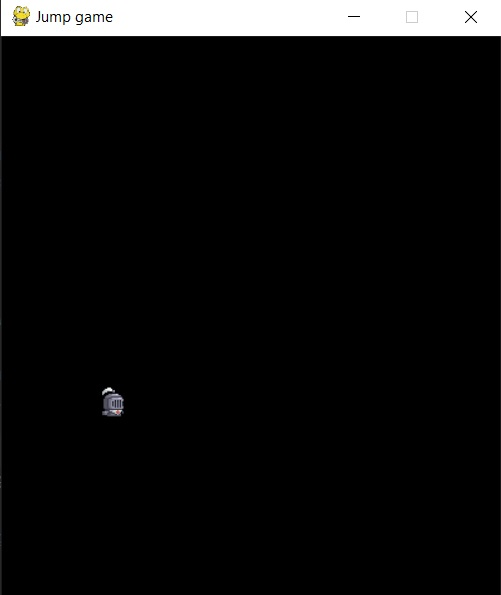
\includegraphics[width=1\linewidth]{Intro_systemtest}
	\caption{Состояние "Intro" при запуске программы}
	\label{Intro_systemtest:image}
\end{figure}

На рисунке \ref{spawn:image} представлен пример начальной позиции игрока(начальное состояние игры).
\begin{figure}[H]
	\centering
	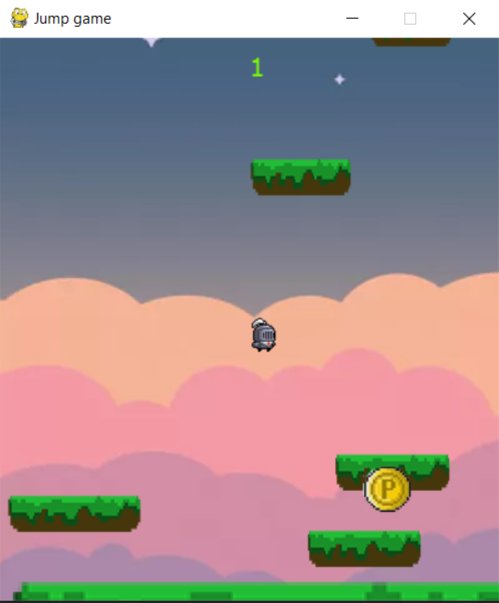
\includegraphics[width=1\linewidth]{spawn}
	\caption{Начало игры}
	\label{spawn:image}
\end{figure}

На рисунке \ref{PlatPoint:image} представлено начисление 1 очка за прыжок на новую платформу.
\begin{figure}[H]
	\centering
	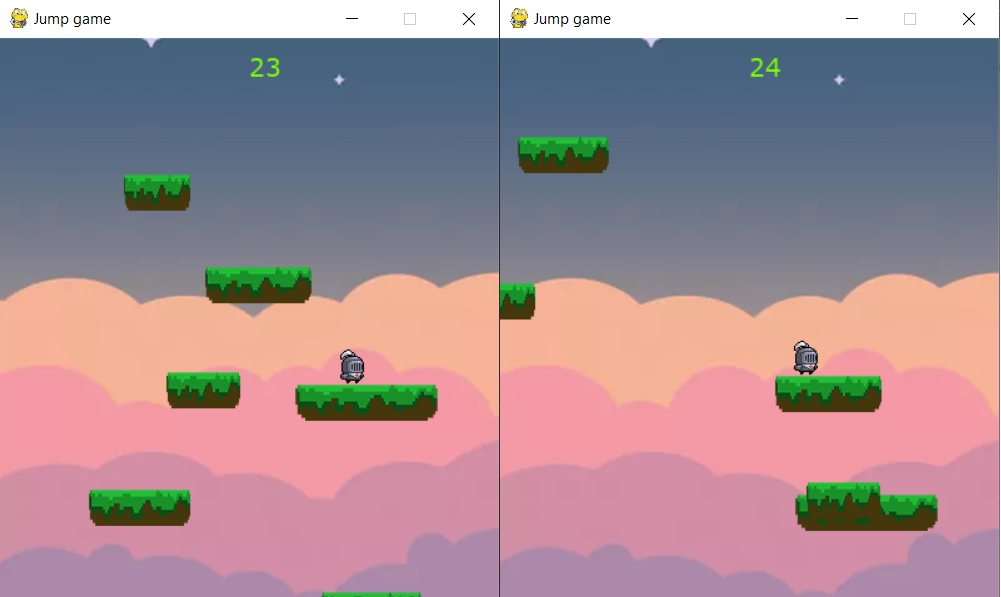
\includegraphics[width=1\linewidth]{PlatPoint}
	\caption{Начисление очков за передвижение по платформам}
	\label{PlatPoint:image}
\end{figure}

На рисунке \ref{TakeCoin:image} представлен пример начисления 5 очков за сбор монетки.
\begin{figure}[H]
	\centering
	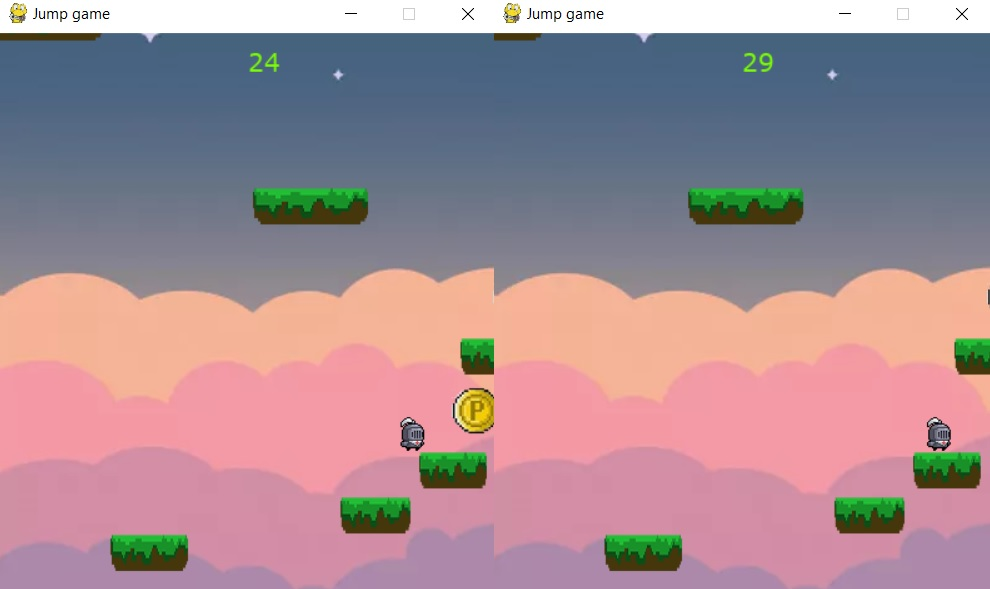
\includegraphics[width=1\linewidth]{TakeCoin}
	\caption{Начисление очков за сбор монеток}
	\label{TakeCoin:image}
\end{figure}

На рисунке \ref{SixPlat:image} представлена постоянная отрисовка 6 платформ.В примере персонаж стоит на платформе 1 и прыгает на платформу 3, после этого платформы 4,5,6 находившиеся снизу ушли за экран, были удалены, а сверху появились новые платформы 4,5,6.
\begin{figure}[H]
	\centering
	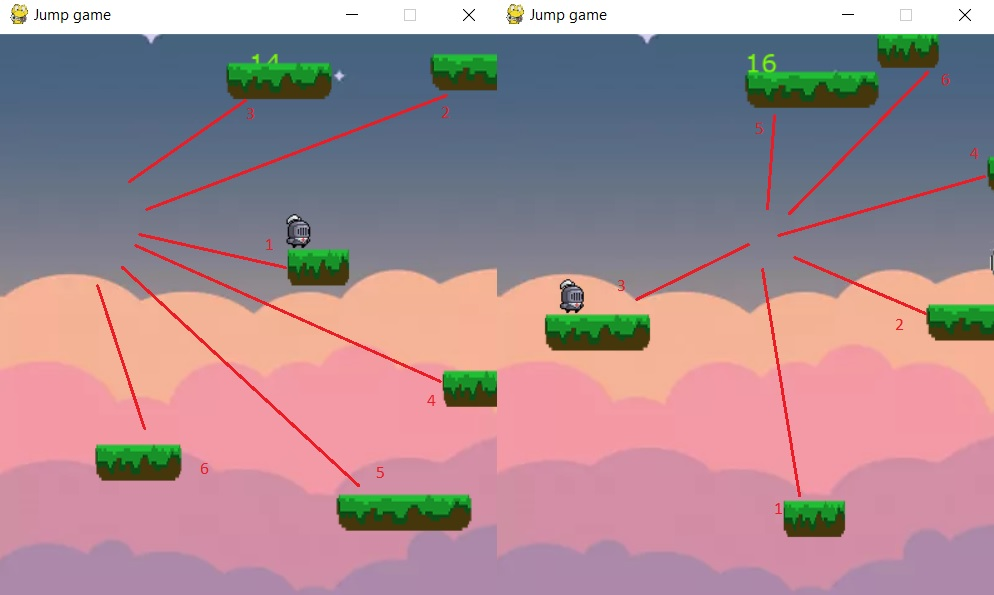
\includegraphics[width=1\linewidth]{SixPlat}
	\caption{Пример постоянной отрисовки 6 платформ}
	\label{SixPlat:image}
\end{figure}

На рисунке \ref{Death:image} представлен пример работы сценария "End Game".
\begin{figure}[H]
	\centering
	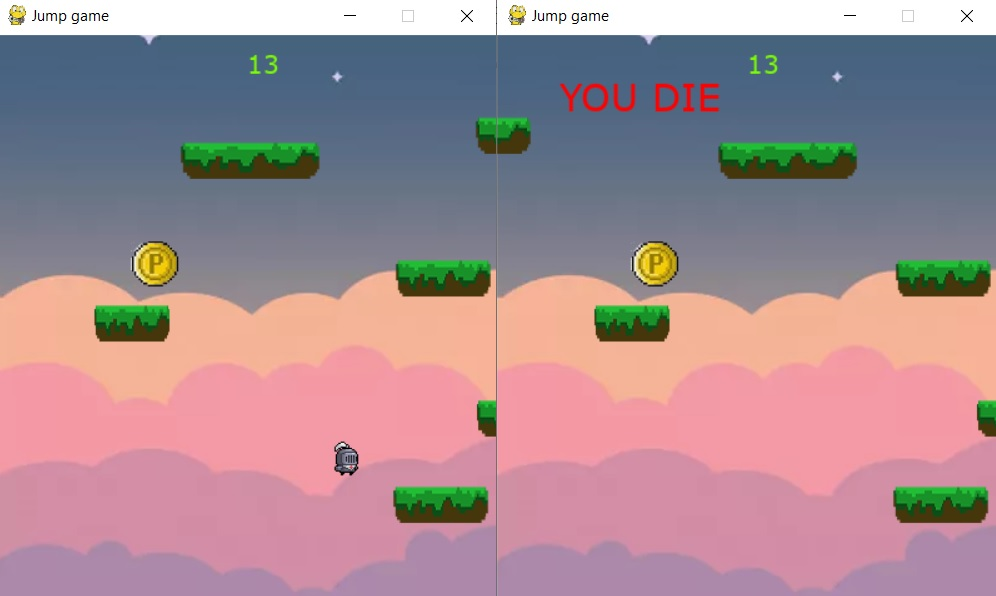
\includegraphics[width=1\linewidth]{Death}
	\caption{Пример работы сценария "End Game"}
	\label{Death:image}
\end{figure}

На рисунке \ref{DeathIntro:image} представлен пример работы смены сценария "End Game" на сценарий "Intro".
\begin{figure}[H]
	\centering
	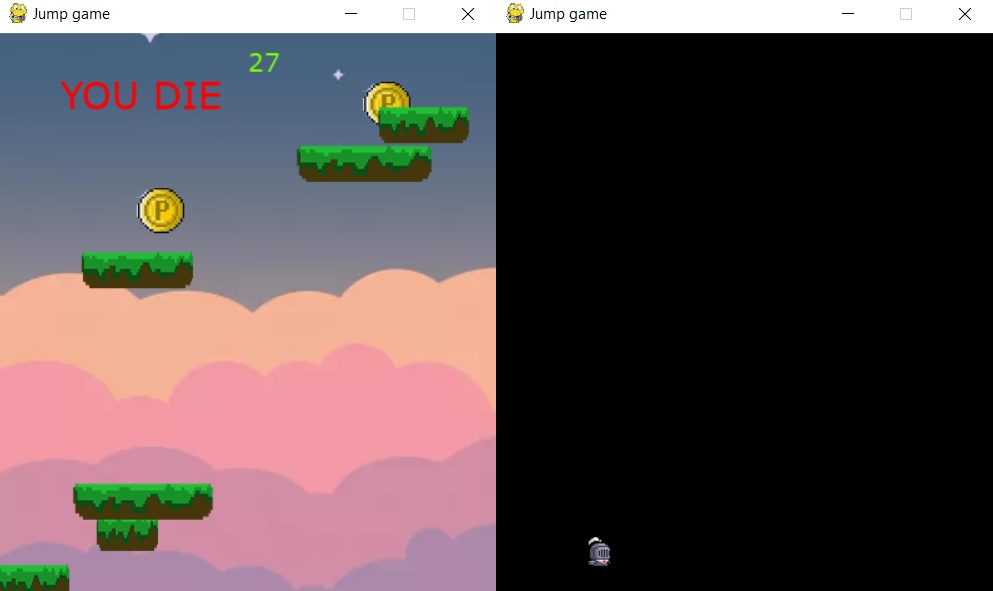
\includegraphics[width=1\linewidth]{DeathIntro}
	\caption{Пример смены сценариев}
	\label{DeathIntro:image}
\end{figure}

